%!TeX root $\leftarrow$ ./00.ppgcc-2020.tex

\section{Implementação com MPI}

Com os desafios de distribuição e memória encontrados nas implementações
preliminares, optou-se por tomar mais controle sobre estes aspectos para
maximizar o aproveitamento do \emph{hardware} escolhido visto que seus recursos
são limitados.
Para isso escolheu-se implementar a proposta utilizando a \acf{MPI} e linguagem C,
onde tem-se controle fino sobre o uso de memória e distribuição, no entanto
perde-se a perícia incluída nas plataformas tradicionais que oferecem
facilidades e garantias necessárias em contextos de ``produção''
(\emph{software} em execução em um ambiente corporativo, que garante o
funcionamento confiável e contínuo de uma corporação).

O algoritmo \minas original \cite{Faria2016minas} tem uma implementação
companheira\footnote{Disponível em \url{http://www.facom.ufu.br/~elaine/MINAS}}
\cite{Faria2013source}, aqui referida como \refminas, escrita em Java utilizando
os algoritmos base como \emph{K-means} e \emph{CluStream} da biblioteca MOA
\cite{MOA}.
Esta implementação serve de referência para a construção provendo validação dos
resultados e servindo também de comparação básica de desempenho.

Os primeiros pontos de divergência do \mfog e \refminas são o algoritmo de
agrupamento e cálculo de raio.
Enquanto \refminas permite a escolha entre \emph{K-means} e \emph{CluStream} para a
fase \emph{offline} e \emph{online}, \mfog implementa apenas \emph{K-means}.
O cálculo de raio em \refminas é definido com o máximo do conjunto de distância
dos exemplos de um \mcluster ao seu centro, seguindo a Equação \ref{eq:raio_max},
enquanto o \mfog segue a definição em \citeonline{Faria2016minas} utilizando o
desvio padrão dos valores do mesmo conjunto de distâncias multiplicado pelo
parâmetro $f_{raio}$ seguindo a Equação \ref{eq:raio_paper}.

\newcommand{\val}{$\vec{v}\,$\xspace}
Os formatos dos fluxos de dados de entrada e de saída também são notáveis. Como
entrada, o algoritmo da proposta recebe dois fluxos, o principal é o que contém
os exemplos, sendo cada exemplo um vetor de números de dimensão $d$.
O segundo fluxo de entrada consiste de \mclusters representando o modelo inicial
criado e capturado da fase de treinamento \emph{offline}.
A fase de treinamento \emph{offline} foi implementada mas não sofre alteração
com relação ao algoritmo \minas \cite{Faria2016minas} além da execução separada
com conjunto de treinamento similar à definição do fluxo de exemplos principal
com adição de uma dimensão com valor de um caractere marcando a classe conhecida
e saída como um fluxo finito de \mclusters.

O formato do fluxo de saída é definido como a tripla contendo o número de
sequência do exemplo no fluxo de entrada (\emph{uid}), etiqueta de um caractere
atribuída ao exemplo e tempo em milissegundos entre a ingestão (entrada) e saída
do exemplo no sistema.

% - Reprocessamento dos exemplos utilizados para atualização do modelo:
%   - Muda o comportamento do operador de fluxo de `Map` para `Flatmap`, ou seja,
%     requer outro fluxo de saída para a transmissão de padrões novidade (alarmes);
%   - Para reclassificação a definição de raio é modificada de `r $\leftarrow$ f * σ` (fator
%     multiplicando desvio padrão) para `r $\leftarrow$ max(distance)` (distância máxima);
%   - Passível da crítica de *overfitting*. Isto é, este processo pode
%     inflar a métrica de precisão;
%   - **Solução:** *em aberto*;

Para avaliação desta proposta, ela foi construída com a implementação \emph{Open
MPI 4.0.4}\footnote{Documentação em \url{https://www.open-mpi.org/doc/v4.0/}} do
padrão \mpi, seguindo o paradigma de programação paralela \acf{SPMD}.
No paradigma \spmd, uma única versão do programa é inicializada em todos os nós,
para cada instância são passados os parâmetros \texttt{mpiSize} e
\texttt{mpiRank} que representa o número de nós e o índice de cada nó no
cluster.
Neste caso o parâmetro \texttt{mpiRank} é o componentes de múltiplos dados em
\spmd e, como cada nó recebe com um valor diferente, cada nó pode ter um
comportamento diferente.
Neste quesito o Algoritmo \ref{alg:minas-main} mostra exatamente esse
comportamento no ponto de entrada do \mfog, dividido o comportamento de cada nó
de acordo com seu \texttt{mpiRank} em dois tipos: raiz e folha.

% For evaluation purposes, an \mfog implementation was made using MPI .
% The program is organized in a single program multiple data (SPMD)
% programming model, so a single version of the \mfog program was initiated on all
% nodes, being that one of them would perform the root role, while the others ran
% as leaves, the program entry point is illustrated on Algorithm \ref{alg:MFOG}.

\begin{algorithm}[htb]
    \SetKwFunction{nearestCluster}{clusterMaisPróximo}
    \SetKwFunction{clustering}{agrupamento}
    \SetKwFunction{NoveltyDetection}{DetecçãoNovidade}
    \SetKwFunction{handleModelSleep}{moveModeloAntigo}
    \SetKwFunction{removeOldSamples}{removeExemplosAntigos}
    % 
    \SetKwFunction{Mfog}{Mfog}
    \SetKwFunction{Sampler}{Fonte}
    \SetKwFunction{Classifier}{Classificador}
    \SetKwFunction{Detector}{Detector}
    \SetKwFunction{modelReceiver}{AtualizaModelo}
    % 
    \SetKwFunction{now}{agora}
    \SetKwFunction{typeOf}{tipoDe}
    \SetKwFunction{Thread}{Thread}
    \SetKwFunction{Lock}{Trava}
    \SetKwFunction{readLock}{travaLeitura}
    \SetKwFunction{writeLock}{travaEscrita}
    % 
    \SetKwFunction{receive}{recebe}
    \SetKwFunction{send}{envia}
    \SetKwFunction{broadcast}{broadcast}
    % 
    \SetKwData{cleaningWindow}{janelaLimpeza}
    \SetKwData{noveltyDetectionTrigger}{gatilhoDetecçãoNovidade}
    \SetKwData{mpiSize}{mpiSize}
    \SetKwData{mpiRank}{mpiRank}
    \SetKwData{EndOfStream}{FimDeFluxo}
    % 
    \SetKwProg{Function}{Função}{:}{}
    \SetKw{continue}{continue}
    \SetKw{break}{pare}
    \SetKwFor{With}{com}{}{}
    % 
    \SetKwInOut{KwIn}{Entrada}
    \SetKwInOut{KwOut}{Saída}
    \SetKwInOut{KwParams}{Parâmetros}
    \KwParams{\mpiRank, \mpiSize}
    \KwIn{fluxoEntrada}
    \KwOut{fluxoSaída}
    % 
    \Function{\Mfog{fluxoEntrada, fluxoSaída}}{
        Modelo $\leftarrow$ $\emptyset$; trava $\leftarrow$ \textbf{new} \Lock()\;
        \eIf(\emph{raiz}){\mpiRank == 0}{
            \textbf{new} \Thread(\Detector, [fluxoSaída, Modelo, trava])\;
            \Sampler(fluxoEntrada, Modelo, trava)\;
        }(\emph{folha}){
            \textbf{new} \Thread(\modelReceiver, [Modelo, trava])\;
            \Classifier(Modelo, trava)\;
        }
    }
\caption{Sistema M-FOG: ponto de entrada.}
\label{alg:MFOG}
\end{algorithm}

No processo raiz, de \texttt{mpiRank} $= 0$ e com acesso aos fluxos de entrada e
de saída, uma \emph{thread} com a função \texttt{Detector} é iniciada e a função
\texttt{Fonte} chamada.
Nos processos folha, de \texttt{mpiRank} $> 0$, uma \emph{thread} com a função
\texttt{AtualizaModelo} é iniciada e a função \texttt{Classificador} chamada.

A função \texttt{Classificador}, listada no Algoritmo \ref{alg:MFOG-leaf}, é o
centro do sistema e opera com o modelo atualizado e um exemplo recebido como
mensagem do nó raiz.
Esta função calcula as distâncias para todos \mclusters do modelo e encontrando
o mais próximo e verificando se o modelo explica aquele exemplo, se explica o
rótulo do \mcluster mais próximo é atribuído como rótulo do exemplo.
A função \texttt{Classificador}, como as outras, só chega ao seu final se a
mensagem recebida (ou instancia lida no caso da função \texttt{Fonte}) é um
marcador de fim de fluxo (\texttt{FimDeFluxo}, \emph{end of stream, eos}).

A função \texttt{AtualizaModelo}, também listada no Algoritmo
\ref{alg:MFOG-leaf}, recebe novos \mclusters como mensagens do nó raiz,
independente deste \mcluster ser do modelo inicial, novidade ou extensão,
adequadamente travando o acesso ao modelo compartilhado com a \emph{thread}
executando a função \texttt{Classificador}.
Além da trava de acesso à leitura e escrita na implementação a função
\texttt{Classificador} espera por um sinal emitido pela função
\texttt{AtualizaModelo} indicando que o modelo está completo antes de começar a
busca pelo \mclusters mais próximo.

\begin{algorithm}[htb]
    \SetKwFunction{nearestCluster}{clusterMaisPróximo}
    \SetKwFunction{clustering}{agrupamento}
    \SetKwFunction{NoveltyDetection}{DetecçãoNovidade}
    \SetKwFunction{handleModelSleep}{moveModeloAntigo}
    \SetKwFunction{removeOldSamples}{removeExemplosAntigos}
    % 
    \SetKwFunction{Mfog}{Mfog}
    \SetKwFunction{Sampler}{Fonte}
    \SetKwFunction{Classifier}{Classificador}
    \SetKwFunction{Detector}{Detector}
    \SetKwFunction{modelReceiver}{AtualizaModelo}
    % 
    \SetKwFunction{now}{agora}
    \SetKwFunction{typeOf}{tipoDe}
    \SetKwFunction{Thread}{Thread}
    \SetKwFunction{Lock}{Trava}
    \SetKwFunction{readLock}{travaLeitura}
    \SetKwFunction{writeLock}{travaEscrita}
    % 
    \SetKwFunction{receive}{recebe}
    \SetKwFunction{send}{envia}
    \SetKwFunction{broadcast}{broadcast}
    % 
    \SetKwData{cleaningWindow}{janelaLimpeza}
    \SetKwData{noveltyDetectionTrigger}{gatilhoDetecçãoNovidade}
    \SetKwData{mpiSize}{mpiSize}
    \SetKwData{mpiRank}{mpiRank}
    \SetKwData{EndOfStream}{FimDeFluxo}
    % 
    \SetKwProg{Function}{Função}{:}{}
    \SetKw{continue}{continue}
    \SetKw{break}{pare}
    \SetKwFor{With}{com}{}{}
    % 
    \Function{\Classifier{Modelo, trava}}{
        \While{ Verdade }{
            exemplo $\leftarrow$ \receive(TipoExemplo, raiz)\;
            \lIf{exemplo == \EndOfStream}{\break}
            exemplo.rótulo $\leftarrow$ "desconhecido"\;
            \With{\readLock(trava)}{
                (distância, cluster) $\leftarrow$ \nearestCluster(exemplo, Modelo)\;
            }
            \If{distância $<$ cluster.raio}{
                exemplo.rótulo $\leftarrow$ cluster.rótulo\;
            }
            \send(raiz, TipoExemplo, exemplo)\;
        }
    }
    %     \label{alg:MFOG-classifier}
    %     \caption{MFOG: Classifier task.}
    % \end{algorithm}
    % \begin{algorithm}
    \Function{\modelReceiver{Modelo, trava}}{
        \While{ Verdade }{
            cluster $\leftarrow$ \receive(TipoCluster, raiz)\;
            \lIf{cluster == \EndOfStream}{\break}
            \With{\writeLock(trava)}{
                Modelo $\leftarrow$ Modelo $\cup$ cluster\;
            }
        }
    }
    % \label{alg:MFOG-model}
    % \caption{MFOG: model receiver task.}
\caption{Funções dos nós folha do \mfog: Atualização de Modelo e Classificador.}
\label{alg:MFOG-leaf}
\end{algorithm}

A função \texttt{Fonte}, listada no Algoritmo \ref{alg:MFOG-root}, lê uma
instância do fluxo de entrada que pode ser do tipo exemplo ou do tipo cluster.
Se a instância for um exemplo, ele é enviado para um dos nós folha, o nó é
escolhido via balanceamento de carga \emph{round-robin}.
Se a instância for do tipo cluster, o modelo compartilhado com a \emph{thread}
executando a função \texttt{Detector} é travado para leitura e escrita e
atualizado e o novo cluster é enviado para todas os nós folhas.

Enquanto a função \texttt{Fonte} gerencia a entrada de dados, a função
\texttt{Detector} gerencia a saída de dados e, como tem acesso aos exemplos já
classificados também gerencia o conjunto de desconhecidos.
Se o tamanho do conjunto de desconhecidos atinge um valor mínimo, a função de
detecção de novidade é chamada, os \mclusters representando padrões novidades ou
extensões são adicionados ao modelo e enviados para todos os nós folha.
Além da remoção dos exemplos utilizados para formar \mclusters de novidades e
extensões, exemplos que participaram duas vezes do processo de detecção de
novidade são considerados \emph{outliers} ou ruído e são removidos.

% On the root process, a sampler thread is responsible for distributing the
% sampled flow information (\val) to the classifier nodes, using a round-robin
% load balancing scheme.
% The other thread on the root process is responsible for receiving the
% classification results and for processing the unknown samples in the search for
% novelties.
% The root process functions are illustrated in Algorithm \ref{alg:MFOG-root}.
% Each leaf node runs a model adjustment thread and multiple (up to the number of
% cores) classifier threads. The leaf tasks are illustrated in Algorithm
% \ref{alg:MFOG-leaf}.

\begin{algorithm}[htb]
    \SetKwFunction{nearestCluster}{clusterMaisPróximo}
    \SetKwFunction{clustering}{agrupamento}
    \SetKwFunction{NoveltyDetection}{DetecçãoNovidade}
    \SetKwFunction{handleModelSleep}{moveModeloAntigo}
    \SetKwFunction{removeOldSamples}{removeExemplosAntigos}
    % 
    \SetKwFunction{Mfog}{Mfog}
    \SetKwFunction{Sampler}{Fonte}
    \SetKwFunction{Classifier}{Classificador}
    \SetKwFunction{Detector}{Detector}
    \SetKwFunction{modelReceiver}{AtualizaModelo}
    % 
    \SetKwFunction{now}{agora}
    \SetKwFunction{typeOf}{tipoDe}
    \SetKwFunction{Thread}{Thread}
    \SetKwFunction{Lock}{Trava}
    \SetKwFunction{readLock}{travaLeitura}
    \SetKwFunction{writeLock}{travaEscrita}
    % 
    \SetKwFunction{receive}{recebe}
    \SetKwFunction{send}{envia}
    \SetKwFunction{broadcast}{broadcast}
    % 
    \SetKwData{cleaningWindow}{janelaLimpeza}
    \SetKwData{noveltyDetectionTrigger}{gatilhoDetecçãoNovidade}
    \SetKwData{mpiSize}{mpiSize}
    \SetKwData{mpiRank}{mpiRank}
    \SetKwData{EndOfStream}{FimDeFluxo}
    % 
    \SetKwProg{Function}{Função}{:}{}
    \SetKw{continue}{continue}
    \SetKw{break}{pare}
    \SetKwFor{With}{com}{}{}
    % 
    \Function{\Sampler{fluxoEntrada, Modelo, trava}}{
        dest $\leftarrow$ 1\;
        \ForEach{ {$exemplo_{i}$} $\in$ fluxoEntrada }{
            \If{\typeOf(exemplo) é TipoCluster}{
                \broadcast(TipoCluster, exemplo, raiz)\;
                \With{\writeLock(trava)}{
                    Modelo $\leftarrow$ Modelo $\cup$ exemplo\;
                }
                \continue\;
            }
            % sample.label $\leftarrow$ unknown\;
            \send(dest, TipoExemplo, exemplo)\;
            dest $\leftarrow$ dest $+ 1$\;
            \lIf{dest $>$ \mpiSize}{dest $\leftarrow$ 1}
        }
    }
    %     \label{alg:MFOG-sampler}
    %     \caption{MFOG: sampler Module.}
    % \end{algorithm}
    % \begin{algorithm}
    \Function{\Detector{fluxoSaída, Modelo, trava}}{
        Desconhecidos $\leftarrow \emptyset$;  últimaLimpeza $\leftarrow 0$\;
        \While{ Verdade }{
            exemplo $\leftarrow$ \receive(TipoExemplo, qualquer)\;
            \lIf{exemplo == \EndOfStream}{\break}
            % $out \leftarrow$ exemplo\;
            fluxoSaída.adicione(exemplo)\;
            \If{exemplo.label == unknown}{
                Desconhecidos $\leftarrow$ Desconhecidos $\cup$ exemplo\;
                \If{$|\;Desconhecidos\;| \geq$ \noveltyDetectionTrigger}{
                    novidades $\leftarrow$ \NoveltyDetection(Modelo, *Desconhecidos)\;
                    \With{\writeLock(trava)}{
                        Modelo $\leftarrow$ Modelo $\cup$ novidades\;
                    }
                    \ForEach{ cluster $\in$ novidades }{
                        \broadcast(TipoCluster, cluster, raiz)\;
                    }
                }
                \If{ exemplo.uid $ > $ ( últimaLimpeza $ + $ \cleaningWindow )}{
                    Desconhecidos $\leftarrow$ \removeOldSamples(Desconhecidos, últimaLimpeza)\;
                    últimaLimpeza $ \leftarrow $ exemplo.uid\;
                }
            }
        }
    }
    % \label{alg:MFOG-detector}
    % \caption{MFOG: detector task.}
\caption{Funções do nó raiz do \mfog: Fonte e Detector.}
\label{alg:MFOG-root}
\end{algorithm}

% The overall sequence of interactions is shown in Figure \ref{fig:mfog-mpi-life}.
As interações entre os diferentes módulos e ciclo de vida do sistema é ilustrado
no diagrama de sequencia da Figura \ref{fig:mfog-mpi-life}.

\begin{figure}[htb]
  \centerline{
    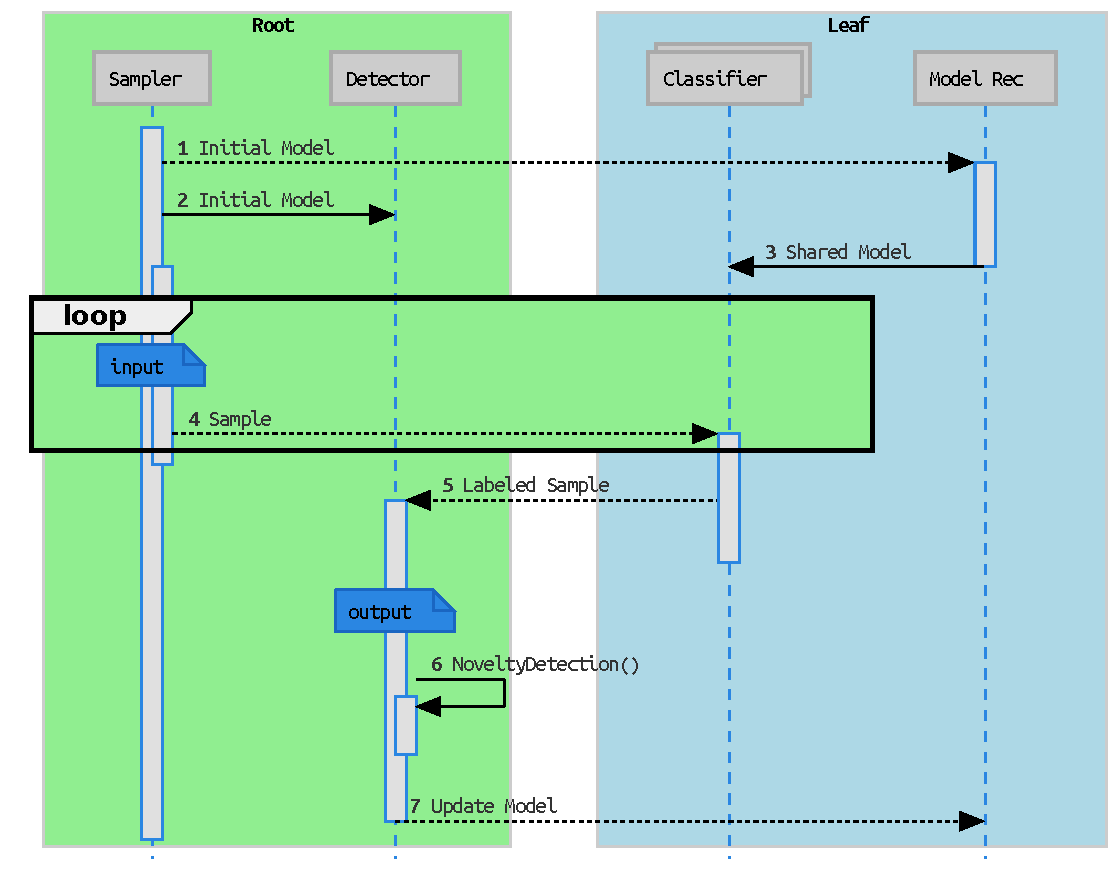
\includegraphics[width=0.9\linewidth,page=1]{figures/lifecycle-uml-svg.pdf}
  }
  \caption{Diagrama UML de Sequência do \mfog: visão geral das linhas de vida.}
  \label{fig:mfog-mpi-life}
\end{figure}

Em suma, a arquitetura do \mfog é composta de múltiplos nós numa névoa que detectam
intrusão numa rede IoT. Para isso os nós da rede processam de forma paralela e
distribuída o cálculo das distâncias e detecção de novidades, sendo assim um
sistema multiprocessado e distribuído. Utiliza-se um único programa com vários
processos por nó, e cada processo recebe um conjunto de dados diferentes
seguindo o paradigma \spmd.
